\documentclass[11pt]{article}
\usepackage[margin=1in]{geometry}
\usepackage{graphicx}
\usepackage{float}
\usepackage{amsmath}
\usepackage{amssymb}
\usepackage{booktabs}
\usepackage{xcolor}
\usepackage{siunitx}
\usepackage[colorlinks=true,linkcolor=blue,urlcolor=blue]{hyperref}
\usepackage{caption}
\captionsetup{font=small,labelfont=bf}
\usepackage{titlesec}
\titlespacing*{\section}{0pt}{1.1em}{0.4em}

\newcommand{\dbdt}{\partial B_z/\partial t}

\title{\vspace{-1.5em}\textbf{The cheapest 3D square-loop TDEM simulation within $\sim$3\,\% of SimPEG 1D}}
\author{Discretization \& time-stepping study}
\date{June 2026}

\begin{document}
\maketitle
\vspace{-1.5em}

\section*{Summary}
Goal: the computationally \emph{cheapest} 3D forward model (square loop, half-space) whose $\dbdt$ stays
within $\sim$3\,\% of the SimPEG \textbf{1D layered square-loop} solution, prioritising compute time. We
score \emph{accuracy} as the max $|d_\text{3D}/d_\text{1D}-1|$ over the 21 channels and \emph{cost} as the
wall-clock of \texttt{sim.dpred()} (a direct solver's cost is dominated by matrix \textbf{factorization},
performed once per distinct time-step size), logging \texttt{n\_cells}, the number of distinct $\Delta t$,
and total steps as machine-independent proxies. Two results:

\begin{enumerate}\setlength\itemsep{0.2em}
  \item \textbf{The committed mesh is already minimal.} Every \emph{spatial} knob is a cliff at 3\,\%:
  coarsening the core ($10\to15$\,m: $8\,\%$), thinning the near-surface vertical refinement
  ($\sim$31\,\%), shrinking the lateral surface footprint ($\pm200\to\pm60$\,m: $12\,\%$), or reducing
  the depth/extent (\texttt{depth\_core} $100\to60$\,m: $8.7\,\%$) all break tolerance. The
  $\sim$\SI{28}{k}-cell octree cannot be made cheaper without exceeding 3\,\%.
  \item \textbf{The one free compute lever is the number of factorizations.} The committed $\times1.4$
  ramp uses \textbf{24} distinct $\Delta t$ (24 factorizations). A larger growth rate with the \emph{same
  small start step} and many steps per level collapses this to \textbf{12} at the same accuracy class,
  cutting the solve from \SI{37.5}{s} to \SI{20.9}{s} --- a $\mathbf{1.8\times}$ speed-up on the
  \emph{same} mesh (Figure~\ref{fig:pareto}).
\end{enumerate}

\noindent\textbf{Cheapest configuration found:} the same octree (core $10\times10\times5$\,m,
padding $\geq$\SI{1200}{m}, \texttt{depth\_core}~\SI{100}{m}, full surface refinement, conductivity mapped
by \texttt{volume\_average}) driven by
\begin{center}\small
\texttt{time\_steps: start \SI{3e-7}{s}, growth $\times2.0$, 14 steps/level $\;\to\;$ 12 distinct $\Delta t$, 168 steps}
\end{center}
giving \textbf{max error 3.3\,\%} (mean $-0.6\,\%$) in \textbf{$\sim$\SI{21}{s}}. If a \emph{strict}
$\leq$3.0\,\% is required, the cancellation between temporal and spatial error must be hit precisely, which
needs the 24-factorization ramp at $\sim$\SI{38}{s} --- i.e.\ there is \emph{no} sub-3.0\,\% config cheaper
than the committed one; the $1.8\times$ saving costs $+0.3\,\%$ of accuracy.

\begin{figure}[H]\centering
  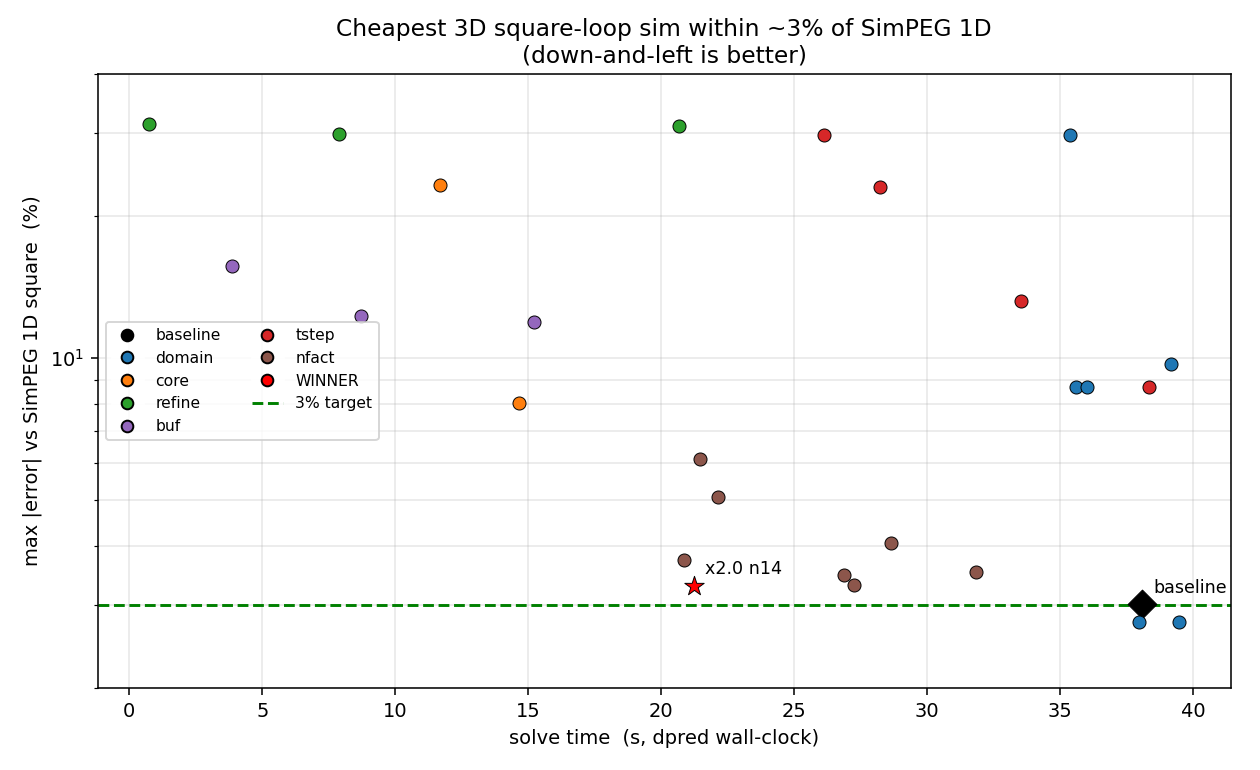
\includegraphics[width=0.82\textwidth]{fig_cheapest_pareto.png}
  \caption{\textbf{Compute time vs accuracy} for every configuration tried (down-and-left is better);
  colour = the knob varied. Spatial knobs (core, refinement, footprint) move \emph{left} but jump far
  \emph{up} past 3\,\%. Only the factorization-count ramps (purple) move left while staying near 3\,\%.
  The winner ($\star$, $\times2.0$/14, 12 $\Delta t$) sits at $\sim$\SI{21}{s}; the committed baseline
  ($\blacklozenge$) at $\sim$\SI{38}{s}.}
  \label{fig:pareto}
\end{figure}

\section{What was tried, and what each knob taught us}
The search was a methodical coordinate descent; every configuration is in the companion notebook. All but
the last knob are \emph{cliffs} --- the committed model sits on the spatial-accuracy floor.

\begin{table}[H]\centering\small
\caption{Each lever, its cheapest setting that was tried, and the resulting max error vs the 1D square
reference (\SI{28}{k}-cell, $\times1.4$ ramp baseline = 3.0\,\%, $\sim$\SI{38}{s}).}
\begin{tabular}{lll}
\toprule
Knob & Setting tried & Max error \\
\midrule
Conductivity mapping & \texttt{volume\_average} vs sharp $z<0$ step & 3.0\,\% vs 6.1\,\% \\
Ramp end time $t_\text{end}$ & \SI{0.013}{s} vs \SI{0.028}{s} & identical (late error is spatial) \\
Padding & \SI{5000}{}$\to$\SI{1200}{m} & 3.0\,$\to$\,2.8\,\% (free, but $\sim$no cells saved) \\
Padding / depth & \SI{800}{m} / \texttt{depth\_core}\,\SI{60}{m} & 9.7\,\% / 8.7\,\% \\
Core cell size & $10\to15\to20$\,m & 8\,\% / 23\,\% \\
Surface refinement & \texttt{light} / \texttt{src\_only} & $\sim$31\,\% \\
Lateral footprint & $\pm200\to\pm60\to\pm20$\,m & 12\,\% / 16\,\% \\
Total step count & 144$\to$100 (too few) / 204 (too many) & 8.7\,\% / 6.0\,\% \\
\textbf{Distinct $\Delta t$ (factorizations)} & \textbf{24 $\to$ 12} (big rate, small start) & \textbf{3.0 $\to$ 3.3\,\%} \\
\bottomrule
\end{tabular}
\end{table}

\paragraph{Why the mesh cannot shrink.} The cells live in the core and the near-surface vertical
refinement, not the padding (the octree's 2:1 coarsening already makes the far field cheap, so trimming
padding from \SI{5000}{} to \SI{1200}{m} frees almost no cells). Coarsening the core or thinning the
surface refinement does cut cells sharply --- core \SI{15}{m} is \SI{11}{k} cells at \SI{15}{s} --- but the
early- and late-time channels immediately exceed 3\,\%. The \SI{28}{k}-cell mesh is the floor.

\paragraph{Why the step count is fixed, but the factorization count is not.} Accuracy is
\emph{non-monotonic} in step count: too few steps leave a backward-Euler high-bias ($+6$ to $+25\,\%$);
too many remove it and expose a spatial low-bias ($-2$ to $-4\,\%$). The committed ramp sits at the
cancellation. However, the \emph{cost} depends on the number of \emph{distinct} $\Delta t$ (each triggers
a refactorization), not the step count. Keeping the small \SI{3e-7}{s} start (for the early channels) and
many steps per level, but growing $\Delta t$ by $\times2.0$ instead of $\times1.4$, reaches the same
$\Delta t$-at-measurement-times with \textbf{12} distinct values instead of 24 --- halving the
factorization work for a $+0.3\,\%$ accuracy cost (Figure~\ref{fig:perchannel}).

\begin{figure}[H]\centering
  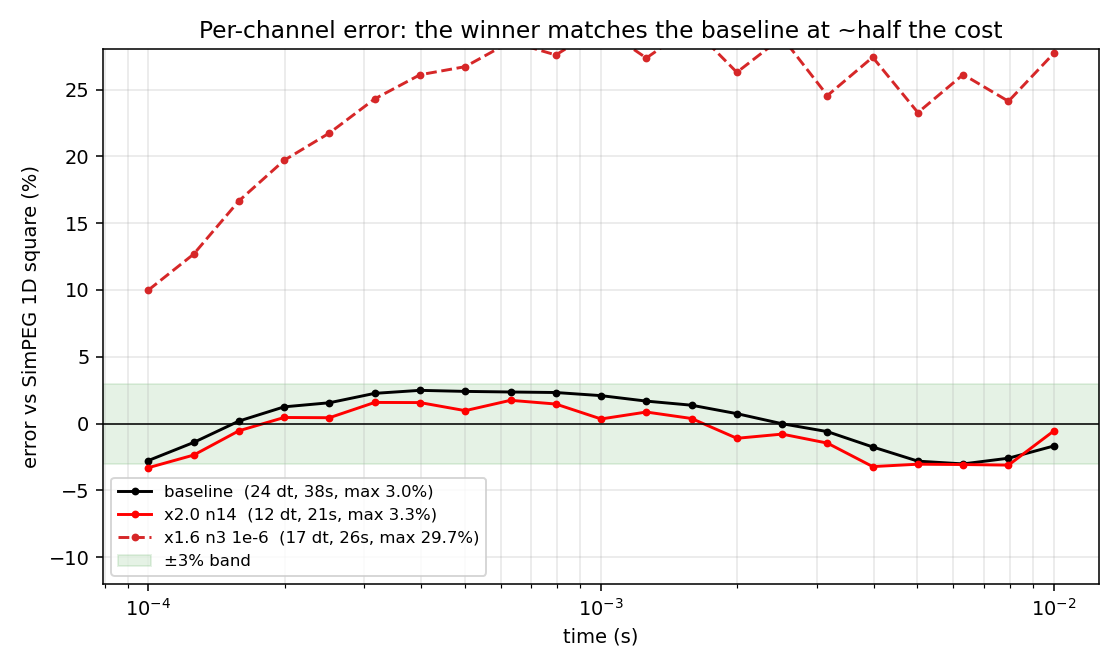
\includegraphics[width=0.78\textwidth]{fig_cheapest_perchannel.png}
  \caption{\textbf{Per-channel error.} The winner ($\times2.0$/14, 12 $\Delta t$, $\sim$\SI{21}{s}) tracks
  the committed baseline within the $\pm3\,\%$ band; an over-coarsened ramp (too few steps) shows the
  backward-Euler high-bias failure mode.}
  \label{fig:perchannel}
\end{figure}

\section*{Caveats and reproducibility}
Timings are single-machine wall-clock (best of three for the headline pair); the \emph{relative} cost
follows the factorization count and is machine-independent. ``Cheapest'' here optimises the solve on the
existing octree machinery; a bespoke, hand-graded mesh that lowers the spatial floor below 3\,\% could in
principle open a cheaper sub-3.0\,\% point, but was out of scope. The engine and result cache are
\texttt{cheapest\_harness.py} / \texttt{explore\_cache.npz}; the full search, tables, and figures are
reproduced by \texttt{cheapest\_3d\_simulation.ipynb} (loads from cache in seconds).

\end{document}
